\documentclass[12pt]{article}

\usepackage{macros}

\title{Lecture 1 for EE127 (Fall 2018): Introduction}
\author{Scribes: Yagna Patel}
\date{8/23/2018}
\begin{document}


\maketitle
\section{Introduction}
The name of the course is Optimization Models. The term \textit{Optimization} is the subject matter of this course. In this course, we view everything as an optimization problem. Optimization is a mathematical language we use to describe the world. The term \textit{Models} refers to the fact that throughout the course, rather than solving for these various models, we will consider them as black boxes. We won't delve too deep into the algorithms. 

\subsection{What is optimization?}
When optimizing something, we generally minimize or maximize some objective, or cost, function. The standard form for an optimization problem is:
\begin{equation*}
\begin{aligned}& \mathbf{p}^*=\underset{\mathbf{x}}{\min}& & f_0(\mathbf{x}) \\& \text{subject to}& & f_i(\mathbf{x}) \leqslant 0, \; i = 1, \ldots, m.\end{aligned}\tag{1}\end{equation*}
where 
\begin{itemize}
\item $\mathbf{x}\in\mathbb{R}^n$ is the decision variable. The decision, or choice, we have to make is encoded into a finite dimensional vector, $\mathbf{x}$. For example, in statistical learning, where our goal is to predict something such as a stock price, demand, etc., $\mathbf{x}$ would be the parameter which helps you make an accurate prediction. In self driving cars, $\mathbf{x}$ could be the speed of the car. 
\item $f_0\,:\,\mathbb{R}^n\to\mathbb{R}$ is the objective, or cost, function. 
\item $f_i\,:\,\mathbb{R}^n\to\mathbb{R}, i=1,\ldots, m$ are the constraints. These constraints, $f_i(\mathbf{x})$, that our decision should satisfy. For example, in the case of self driving cars, if we wanted to restrict our car to drive within a certain speed limit, we could add a constraint for $\mathbf{x}$. 
\item $\mathbf{p}^*$ is the optimal value. Solving an optimization problem essentially means to find a solution, $\mathbf{p}^*$, such that the constraints are satisfied and such that the objective function is minimized. Sometimes, if the constraints are too stringent, the solution may not exist. Essentially, $\mathbf{p}^*$ is a solution to the optimization problem if for all $\mathbf{x}$ such that for every $i$, $f_i(\mathbf{x}) \leqslant 0$, then $f_0(\mathbf{p}^*)\leqslant f_0(\mathbf{x})$.
\end{itemize}
\noindent Note that we can write \textit{any} optimization problem in this standard form (1). For example, if we wanted to maximize our objective function, $\max_\mathbf{x} f_0(\mathbf{x})$ we could instead minimize $\min_\mathbf{x}{\text{-} f_0(\mathbf{x})}$. 


\subsection{Examples of Optimization Problems}
Almost every field of science and engineering has applications of optimization. We will look at a few of those applications.
\subsubsection{Least-Squares Regression}
\begin{figure}[h!]\begin{center}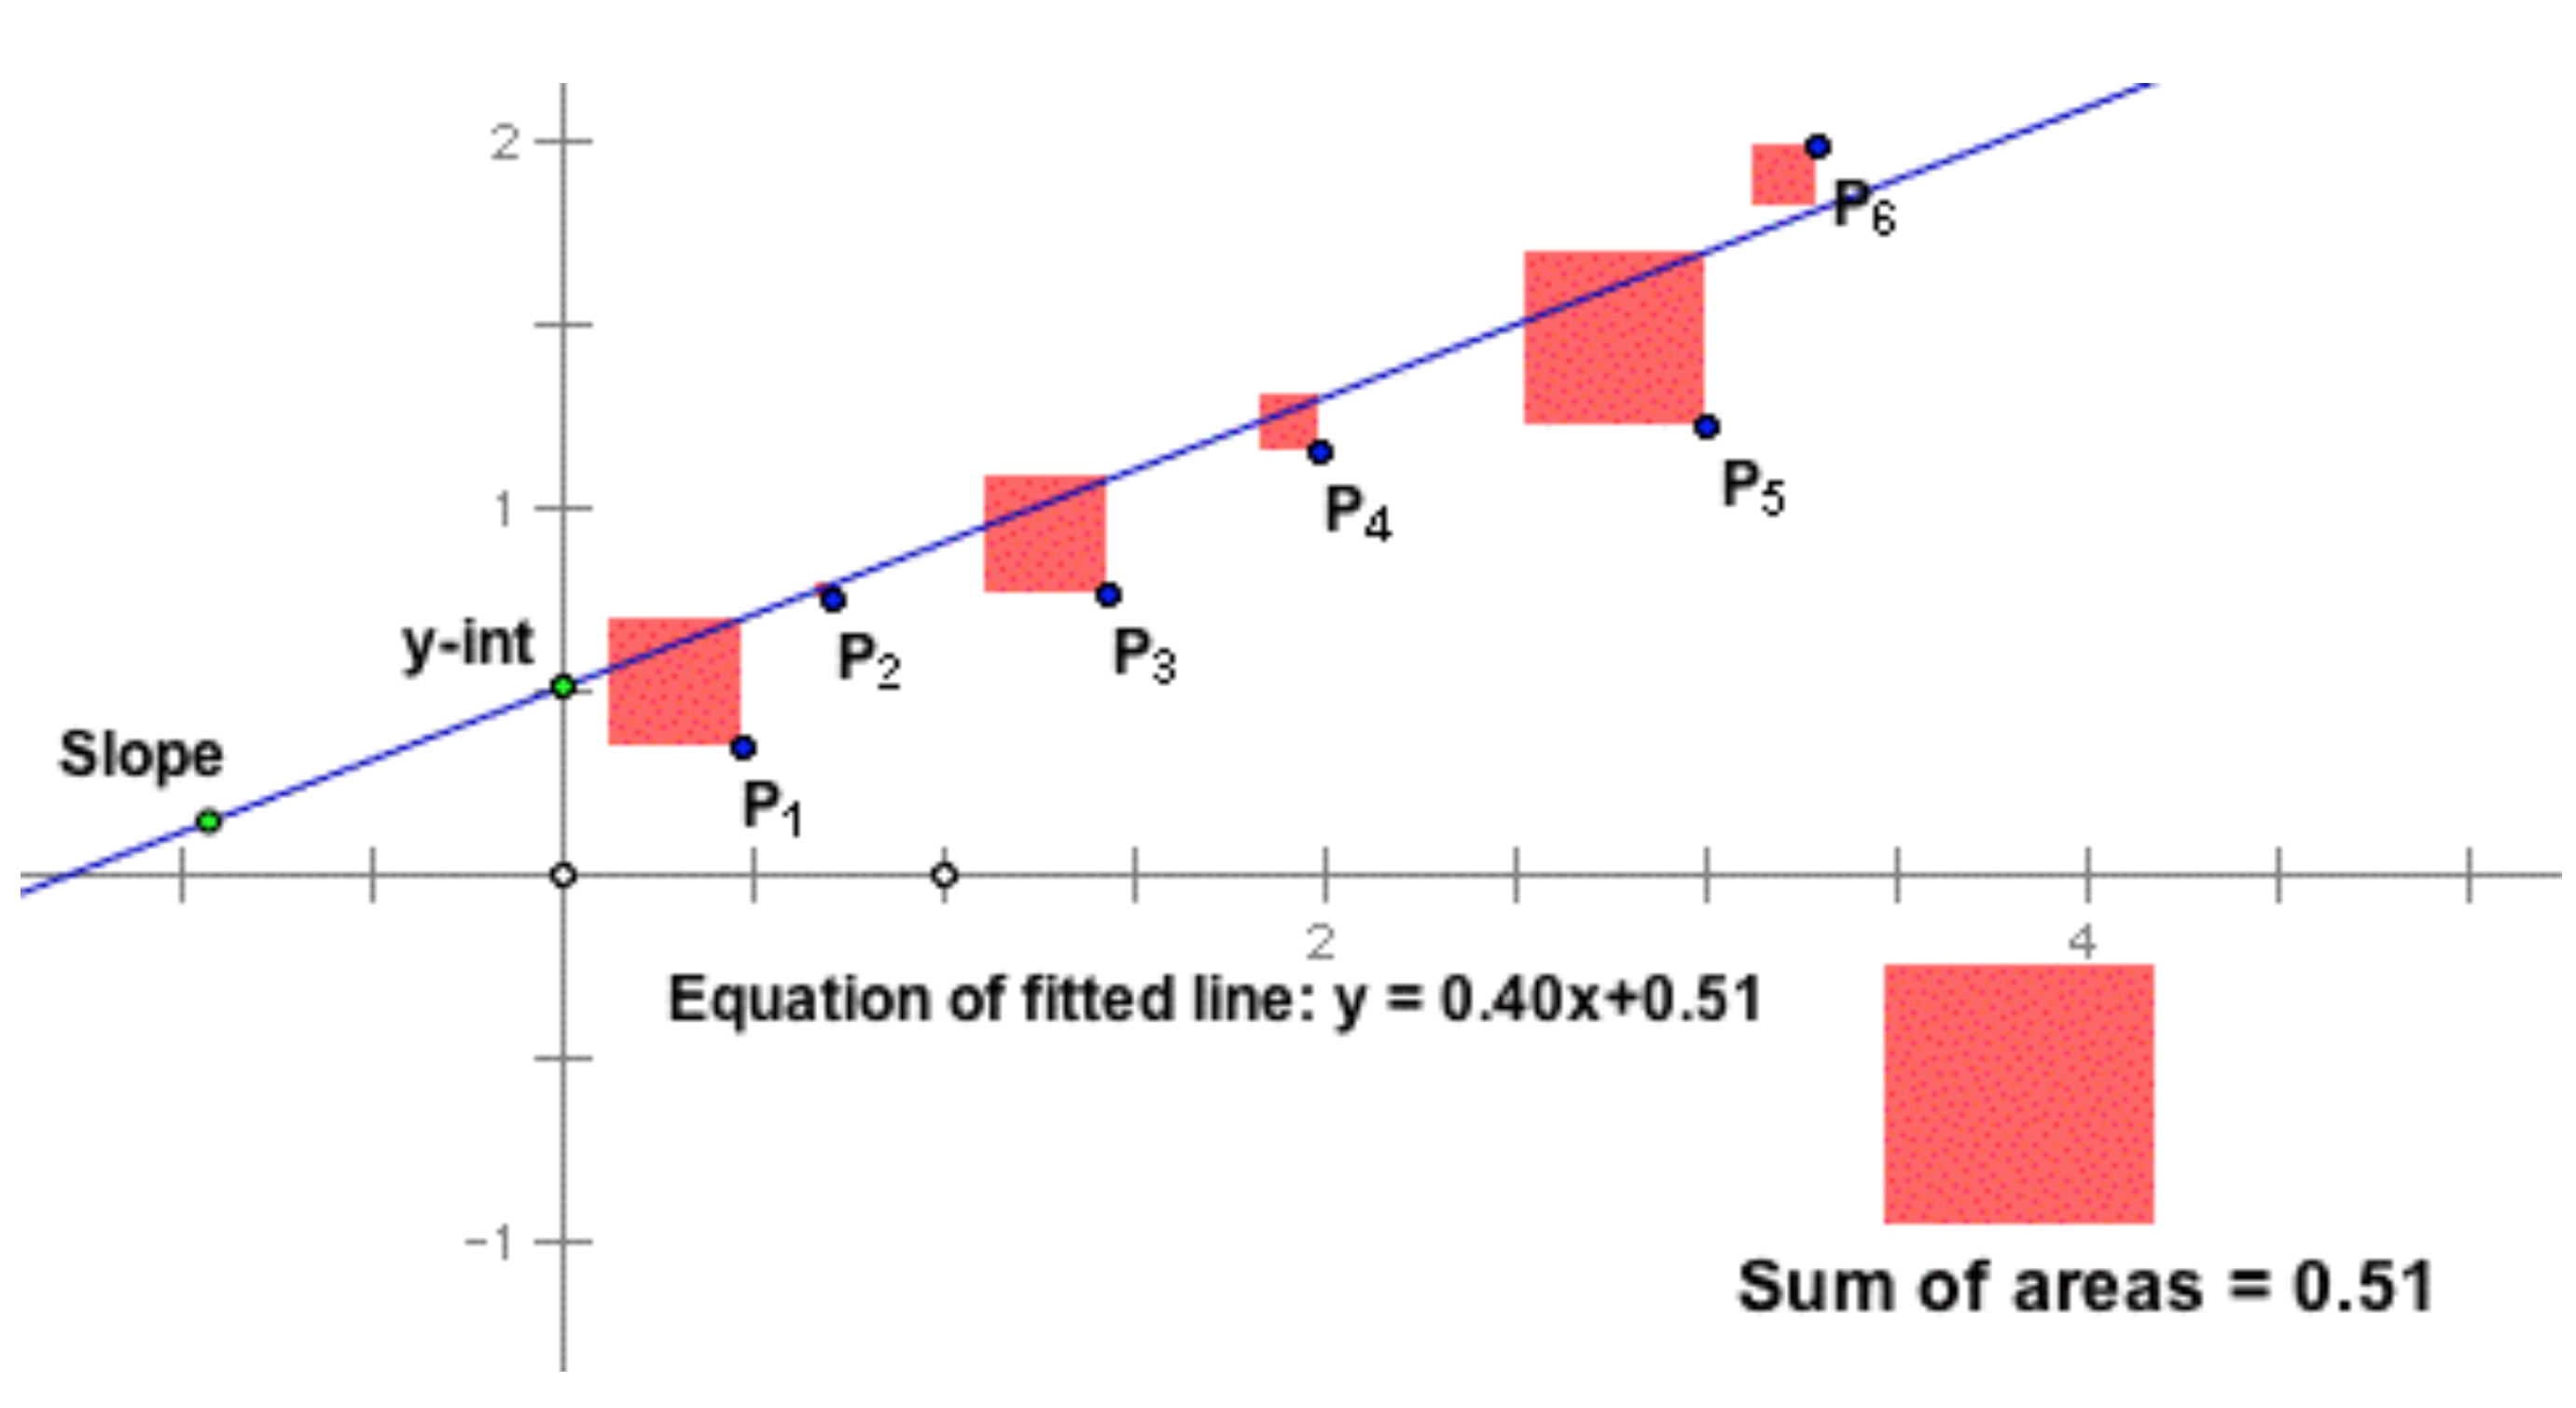
\includegraphics[scale=0.2]{figures/leastsquares}\caption{Least-Squares Example}\end{center}\end{figure}
\noindent One of the oldest optimization problems is the least-squares regression problem. It holds roots back to Gauss's time. This is an example of an optimization problem that doesn't have any constraints. In Figure 1, we see an example of performing least-squares regression on $6$ data points. The goal of least-squares regression is to minimize the sum of the areas for each point for a fitted line. 
\noindent Therefore, the objective function becomes $$f_0(\mathbf{x}) = \sum_{i=1}^m \left(y_i-\mathbf{x}^\top \mathbf{z}^{(i)}\right)^2 = \|\mathbf{y} - \mathbf{Z}\mathbf{x}\|_2^2$$
Note that $\|\cdot\|_2^2$ is the square of the euclidean norm. 
Therefore, our optimization problem is
$$\min_\mathbf{x}f_0(\mathbf{x})$$ 
where
\begin{itemize}
\item $\mathbf{Z}\in\mathbb{R}^{m\times n}$ is a matrix of input data points. 
\item $\mathbf{y}\in\mathbb{R}^m$ is a \textit{response} vector. Response vectors are essentially output vectors.
\item $\mathbf{x}^\top \mathbf{z}$ is the scalar product, $z_1x_1 + \ldots + z_nx_n$ between the two vectors $x,z\in\mathbb{R}^n$. $\mathbf{x}^\top \mathbf{z}$ is the fitted line. Once we have figured out the best fit line, the line is encoded into $\mathbf{x}$. $\mathbf{x}$ is the \textit{decision} variable; it allows us to make a precise prediction. 
\end{itemize}
Now, if we get a new point, we can use the fitted line (blue line in Figure 1) to make a prediction. 
\subsubsection{Linear Classification}
\begin{figure}[h!]\begin{center}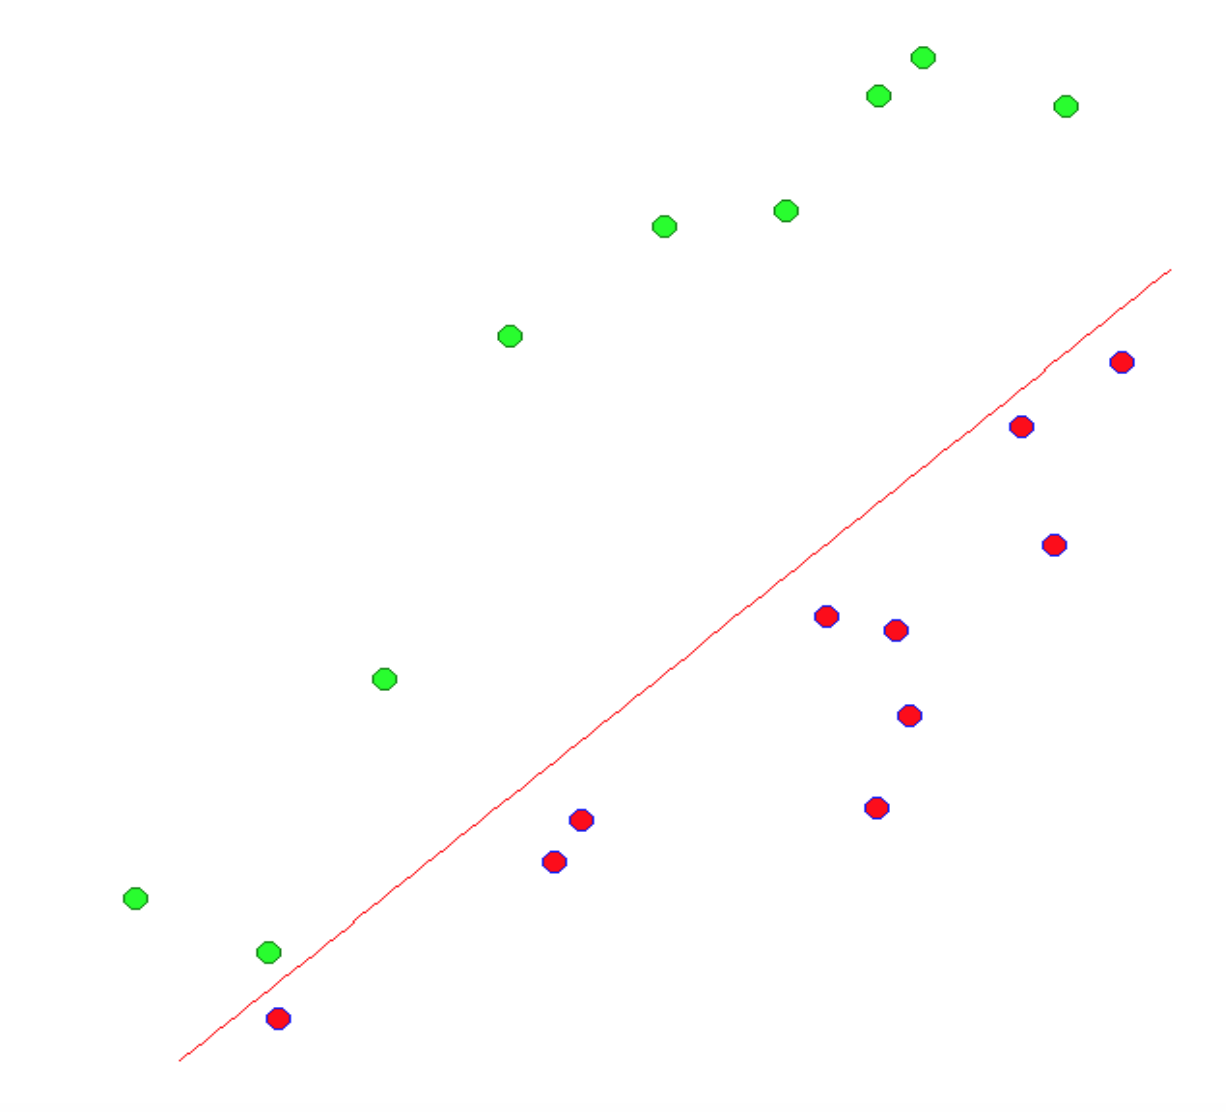
\includegraphics[scale=0.3]{figures/svm}\caption{SVM Example}\end{center}\end{figure}
\noindent Another example of an optimization problem is linear classification. Suppose that, in Figure 2, each of the points are in $40,000$ dimensions, and the red points represent patients who have \textit{not} developed diabetes over the past 6 months, and the green points represent patients who have developed diabetes. Now, suppose that a new patient comes to us. How can we predict whether or not this patient will have diabetes? 

\noindent This is a linear classification problem. We want to find a boundary which best separates the green points and the red points. One way to approach this problem is to use Support Vector Machines (SVMs). 

\noindent The optimization problem for an SVM is  $$\min_{\mathbf{x},\mathbf{b}} \sum_{i=1}^m \max\left\{0, 1-y_i(\mathbf{x}^\top\mathbf{z}^{(i)} + \mathbf{b})\right\}$$
where
\begin{itemize}
\item $\mathbf{z}^{(i)}\in\mathbb{R}^n,i=1,\ldots,m$ are input data points.
\item $\mathbf{y}\in\{-1,1\}^m$ is a binary response vector.
\item $\mathbf{x}^\top\mathbf{z}+\mathbf{b} = 0$ defines a \textit{separating hyperplane} in data space.
\end{itemize}
Now, in order to predict whether the patient will have diabetes, we can look at the sign of the hyperplane $\mathbf{x}^\top\mathbf{z}+\mathbf{b}$. This will tell us which side of the hyperplane the point lies, which in turn tells us whether or not the patient will have diabetes.

\noindent Notice that this wasn't a least-squares problem. It is different from a least-squares problem in that we are instead minimizing a convex function. Simply put, a convex function is a bowl-shaped function.
\subsubsection{Further Examples}
See \href{https://bcourses.berkeley.edu/courses/1473158/files/73475329/download?wrap=1}{Lecture 1 slides} for more examples of optimization problems.
\newpage
\section{Optimization Problems}
Recall the general structure of an optimization problem from equation (1). Let's look at some definitions that will prove useful when dealing with optimization problems.
\subsection{Definitions}
\begin{definition}
A point $\mathbf{x}$ is \textbf{feasible} if $\mathbf{x}\in\text{dom } f_0$ and $\mathbf{x}$ satisfies all the constraints.
\end{definition}
\noindent Given that $f_0$ is our objective function, a point $x$ is said to be feasible for an optimization problem, if it is in the domain of $f_0$ and it satisfies all the constraints of the optimization problem. The set of all such feasible $x$ is called a \textbf{feasible set}. If a point is not feasible, it is \textbf{infeasible}.
\begin{definition}
A feasible point $\mathbf{x}$ is \textbf{optimal} if $f_0(\mathbf{x})=\mathbf{p}^*$.
\end{definition}
\noindent The set of all such optimal $\mathbf{x}$ is called an \textbf{optimal set}.
\begin{figure}[h!]\begin{center}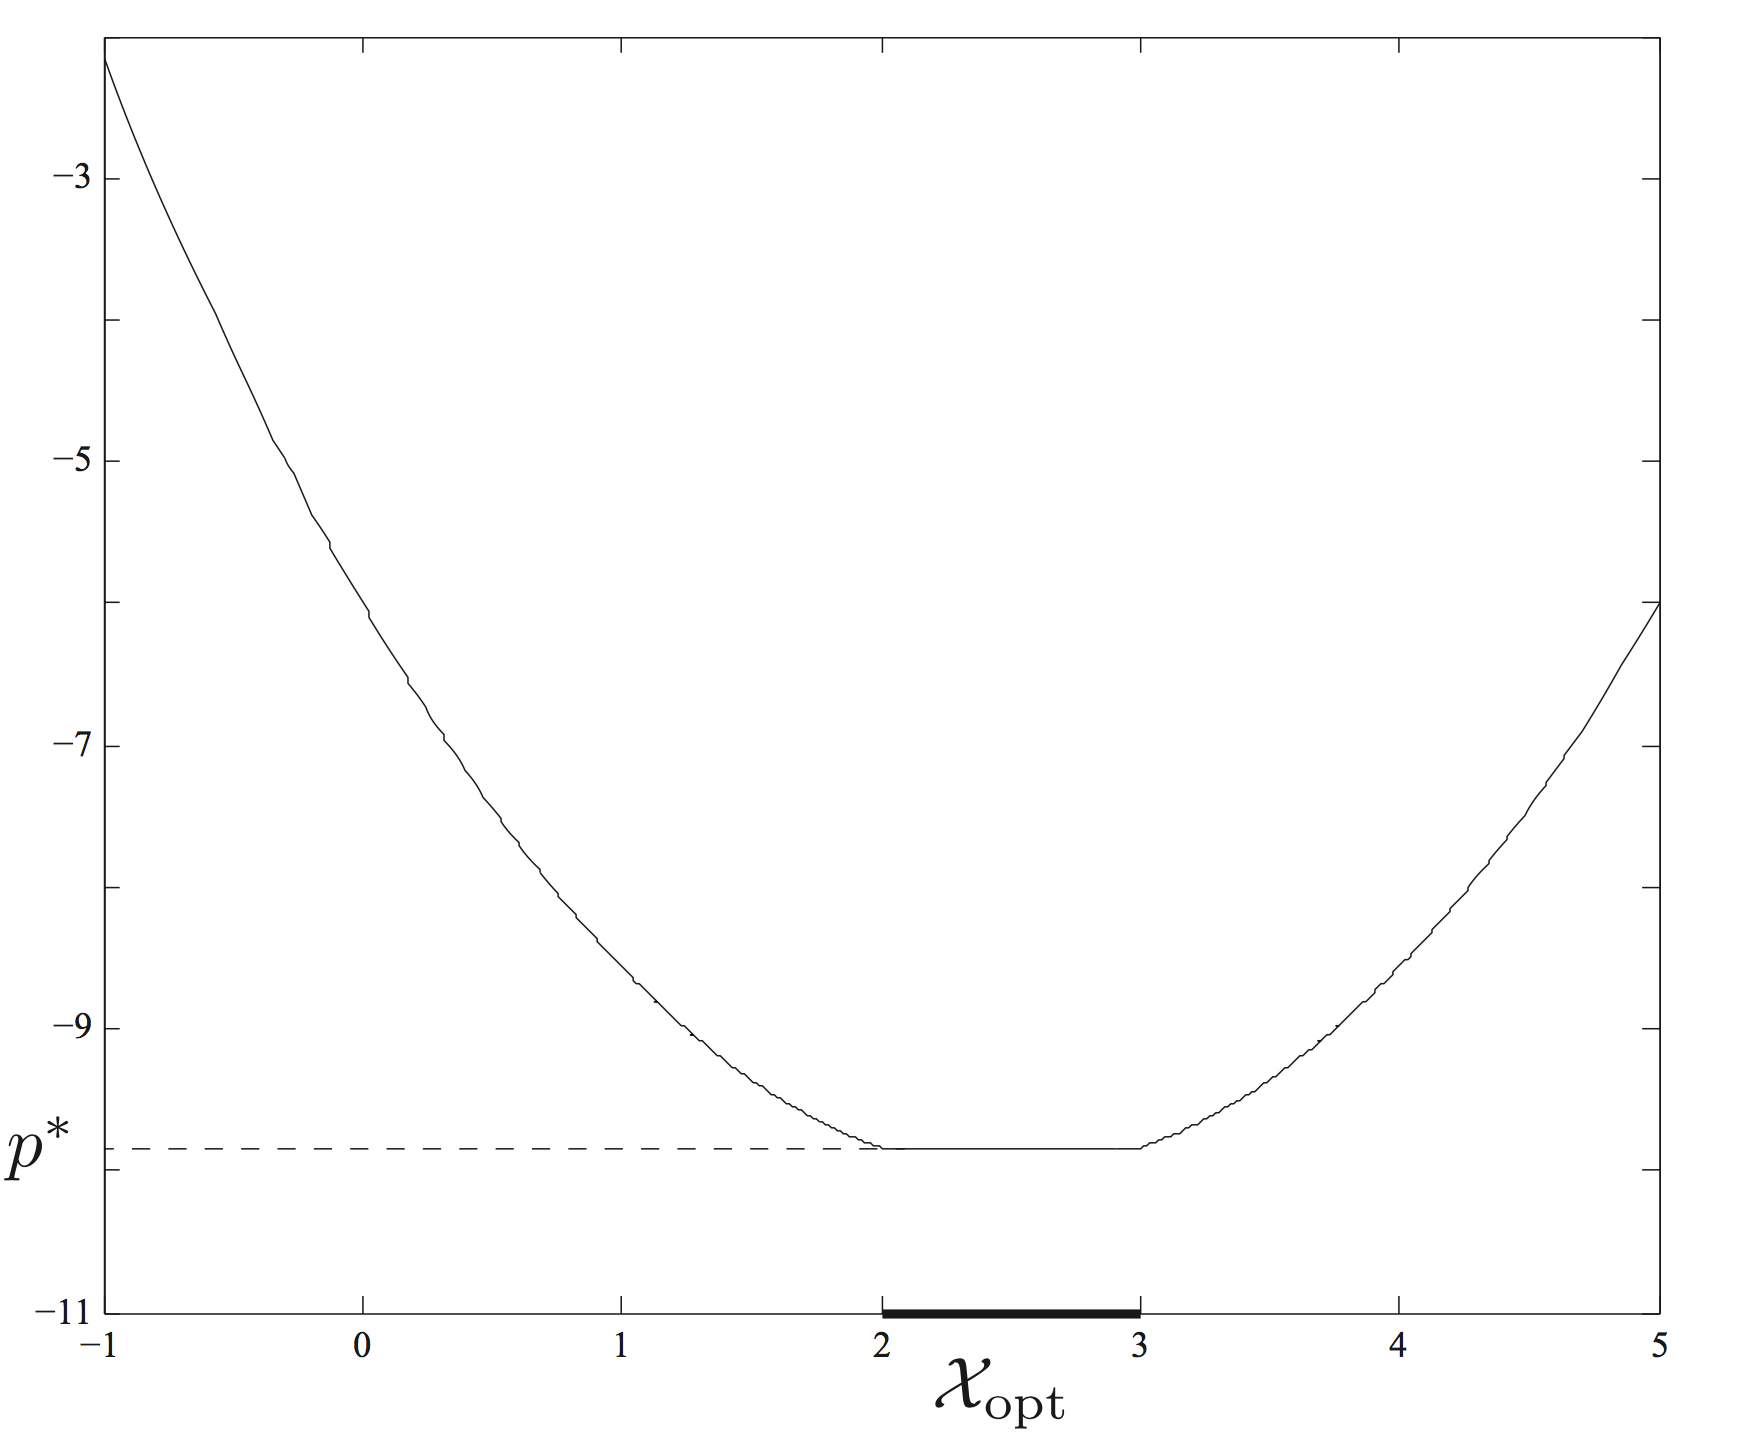
\includegraphics[scale=0.3]{figures/optimalset}\caption{Optimal Set Example}\end{center}\end{figure}

\noindent Notice that in Figure 3 the optimal set is $\chi_{\text{opt}}=[2,3]$. All the points in $[2,3]$ achieve a global minimum value of $\mathbf{p}^*=-9.84$
\begin{definition}
A feasible point $\mathbf{x}$ is $\epsilon$-suboptimal if $f_0(\mathbf{x})\leqslant \mathbf{p}^* + {\epsilon}$.
\end{definition}
\noindent The set of all such $\epsilon$-suboptimal points forms an $\epsilon$-suboptimal set.
\begin{definition}
A point $\mathbf{z}$ is locally optimal if there exists an $R>0$ such that $\mathbf{z}$ is optimal for 
\begin{equation*}
\begin{aligned}& \underset{\mathbf{x}}{\min}& & f_0(\mathbf{x}) \\& \text{subject to}& & f_i(\mathbf{x}) \leqslant 0, \; i = 1, \ldots, m \\ & & &  \|x_i-z_i\|_2\leqslant R , \; i = 1, \ldots, n.\end{aligned}\end{equation*}
\end{definition}
\noindent Consider the following graph:
\begin{figure}[h!]\begin{center}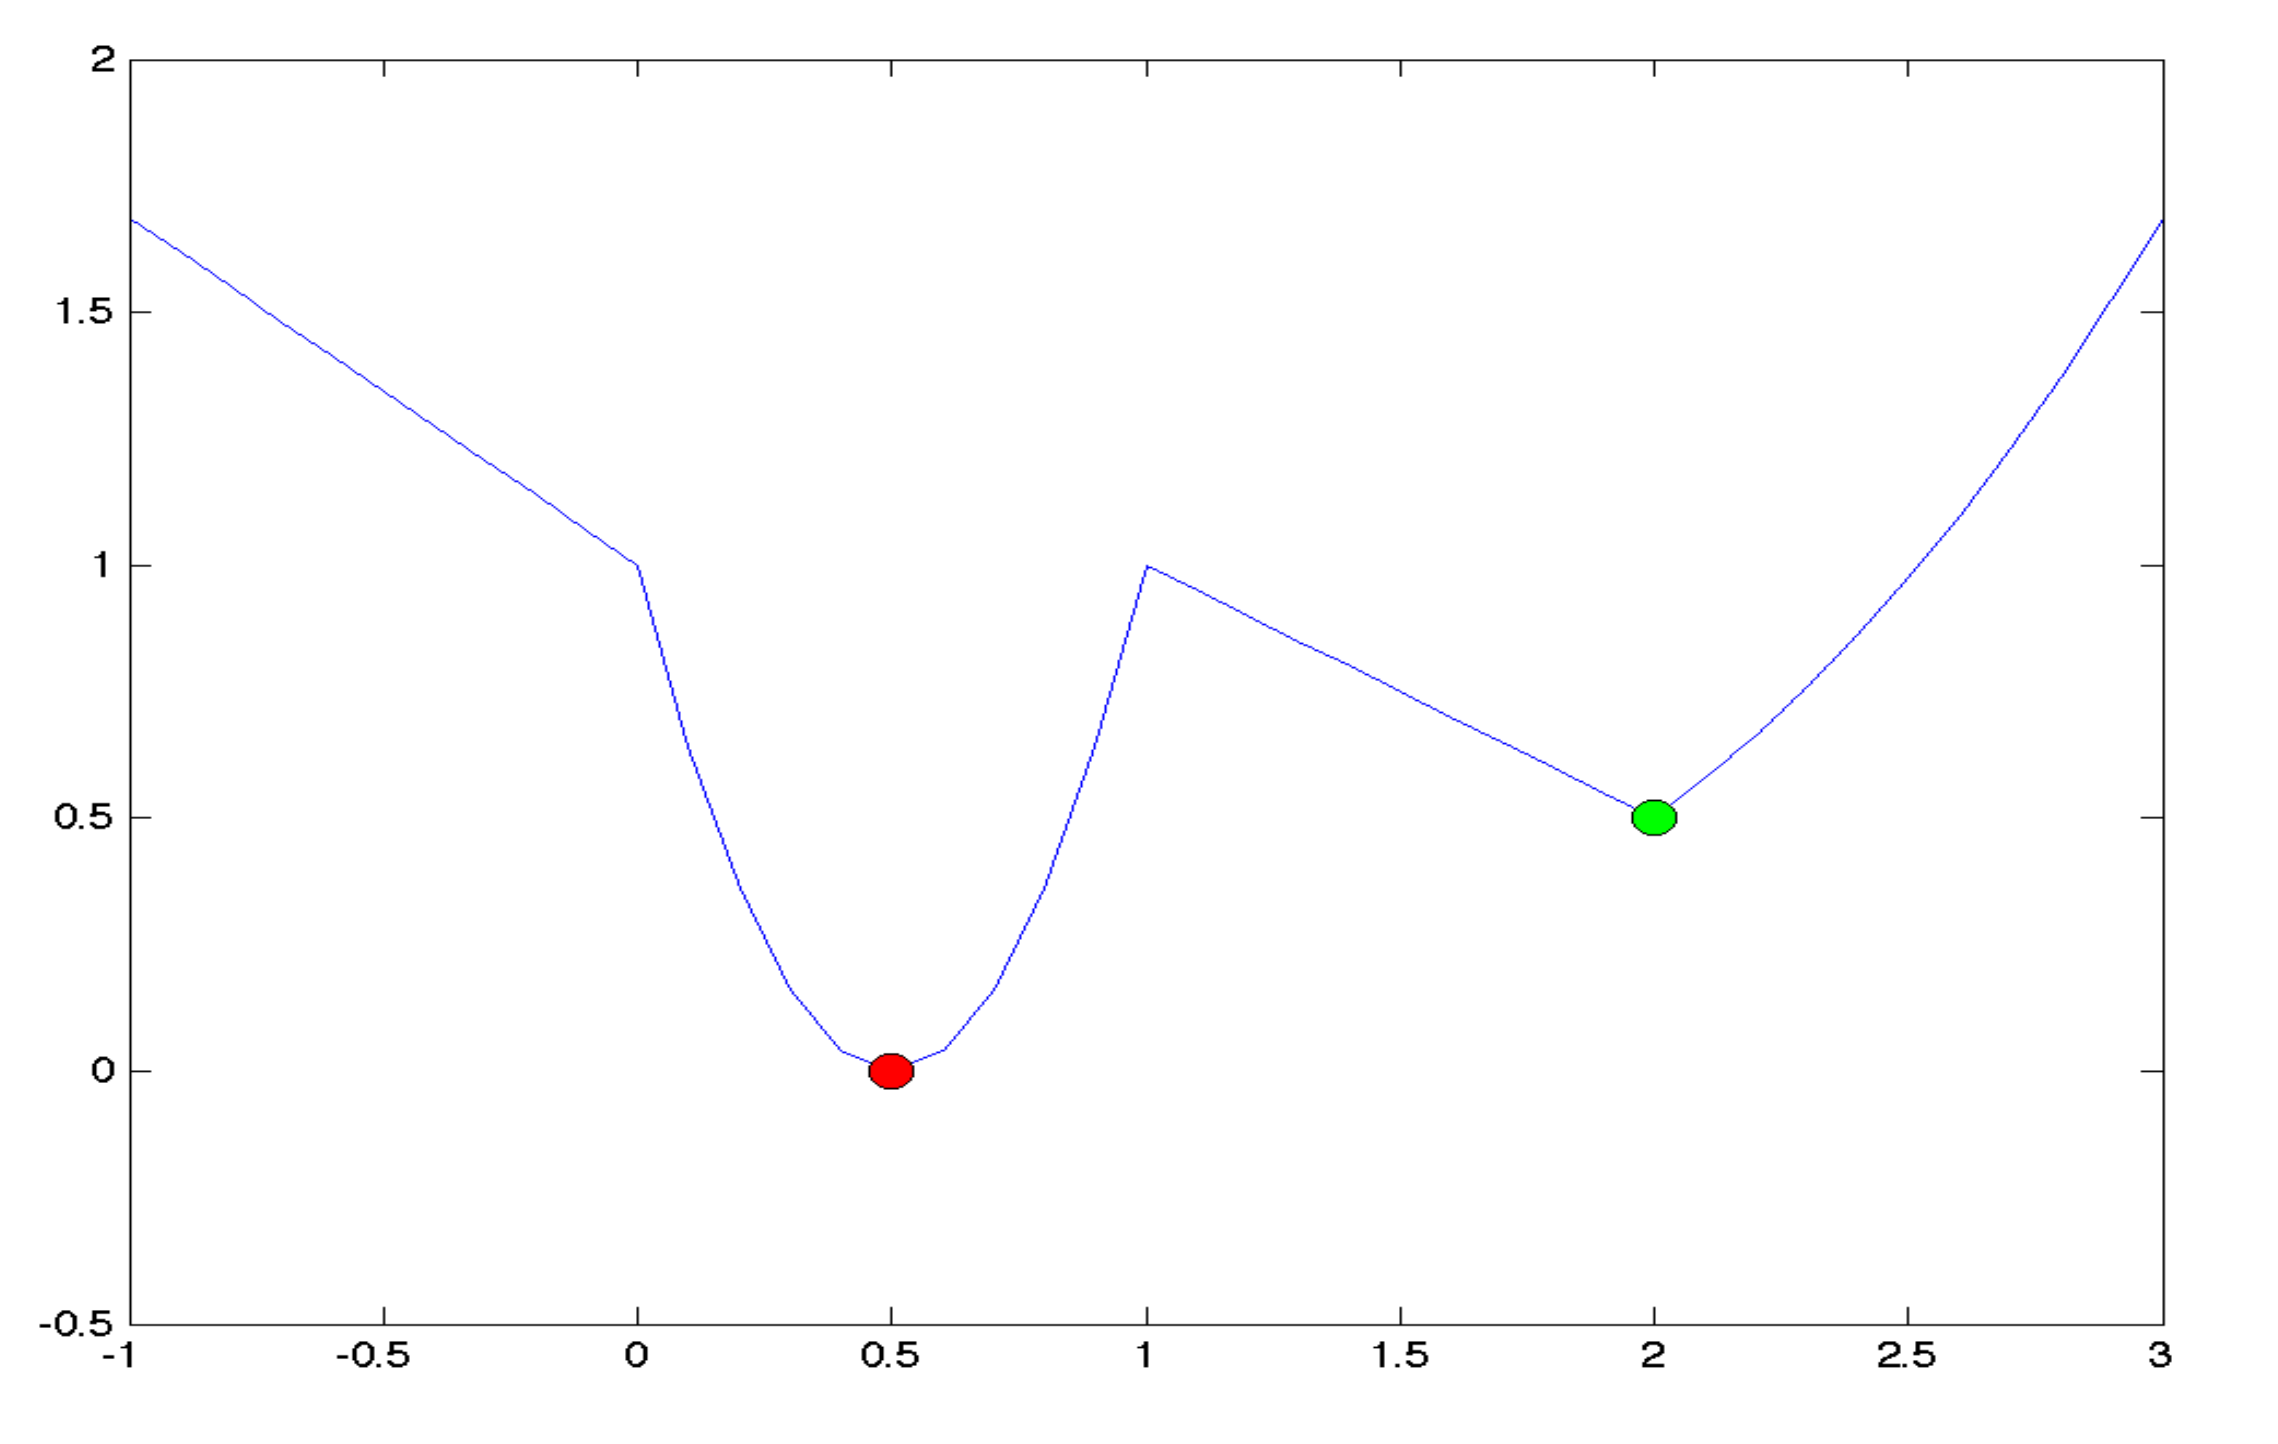
\includegraphics[scale=0.3]{figures/localminimum}\caption{Local/Global Minimum Graph}\end{center}\end{figure}

\noindent In Figure 4 we see the graph of a function of one variable. Now, notice the two points, the green point and the red point. Suppose we run an algorithm to find the minimum of a function, and suppose that our algorithm returned the green point. Now, the green point is nice since locally it is better than it's neighbors. However, as we grow our neighborhood, we see that it isn't the best local minimum. Instead, the red point gives the global minimum of the function. In practice, using either minima could yield very different results. For example, in deep learning, if we have constraints and our algorithm find such a local minimum, it could fail to find a feasible point even though there may exist one. However, for most problems in deep learning, they are unconstrained. Therefore, it isn't really a problem if we don't find the global minimum.
\begin{definition}
A $t$-level set of a function $f$ is defined as $$L_t(f):=\{x\in\mathbb{R}^n\,:\,x\in\mathbb{R}^n, t=f(x)\}$$
\end{definition}
\begin{definition}
A $t$-sublevel set of a function $f$ is defined as $$L_t(f):=\{x\in\mathbb{R}^n\,:\,x\in\mathbb{R}^n, t\geqslant f(x)\}$$
\end{definition}
\begin{example}
Consider the optimization problem
\begin{equation*}
\begin{aligned}& \underset{\mathbf{x}}{\min}& & 0.9x_1^2-0.4x_1x_2-0.6x_2^2-6.4x_2-0.8x_2 \\& \text{subject to}& & -1\leqslant x_1\leqslant 2, 0\leqslant x_2\leqslant 3.\end{aligned}\end{equation*}
\begin{figure}[h!]\begin{center}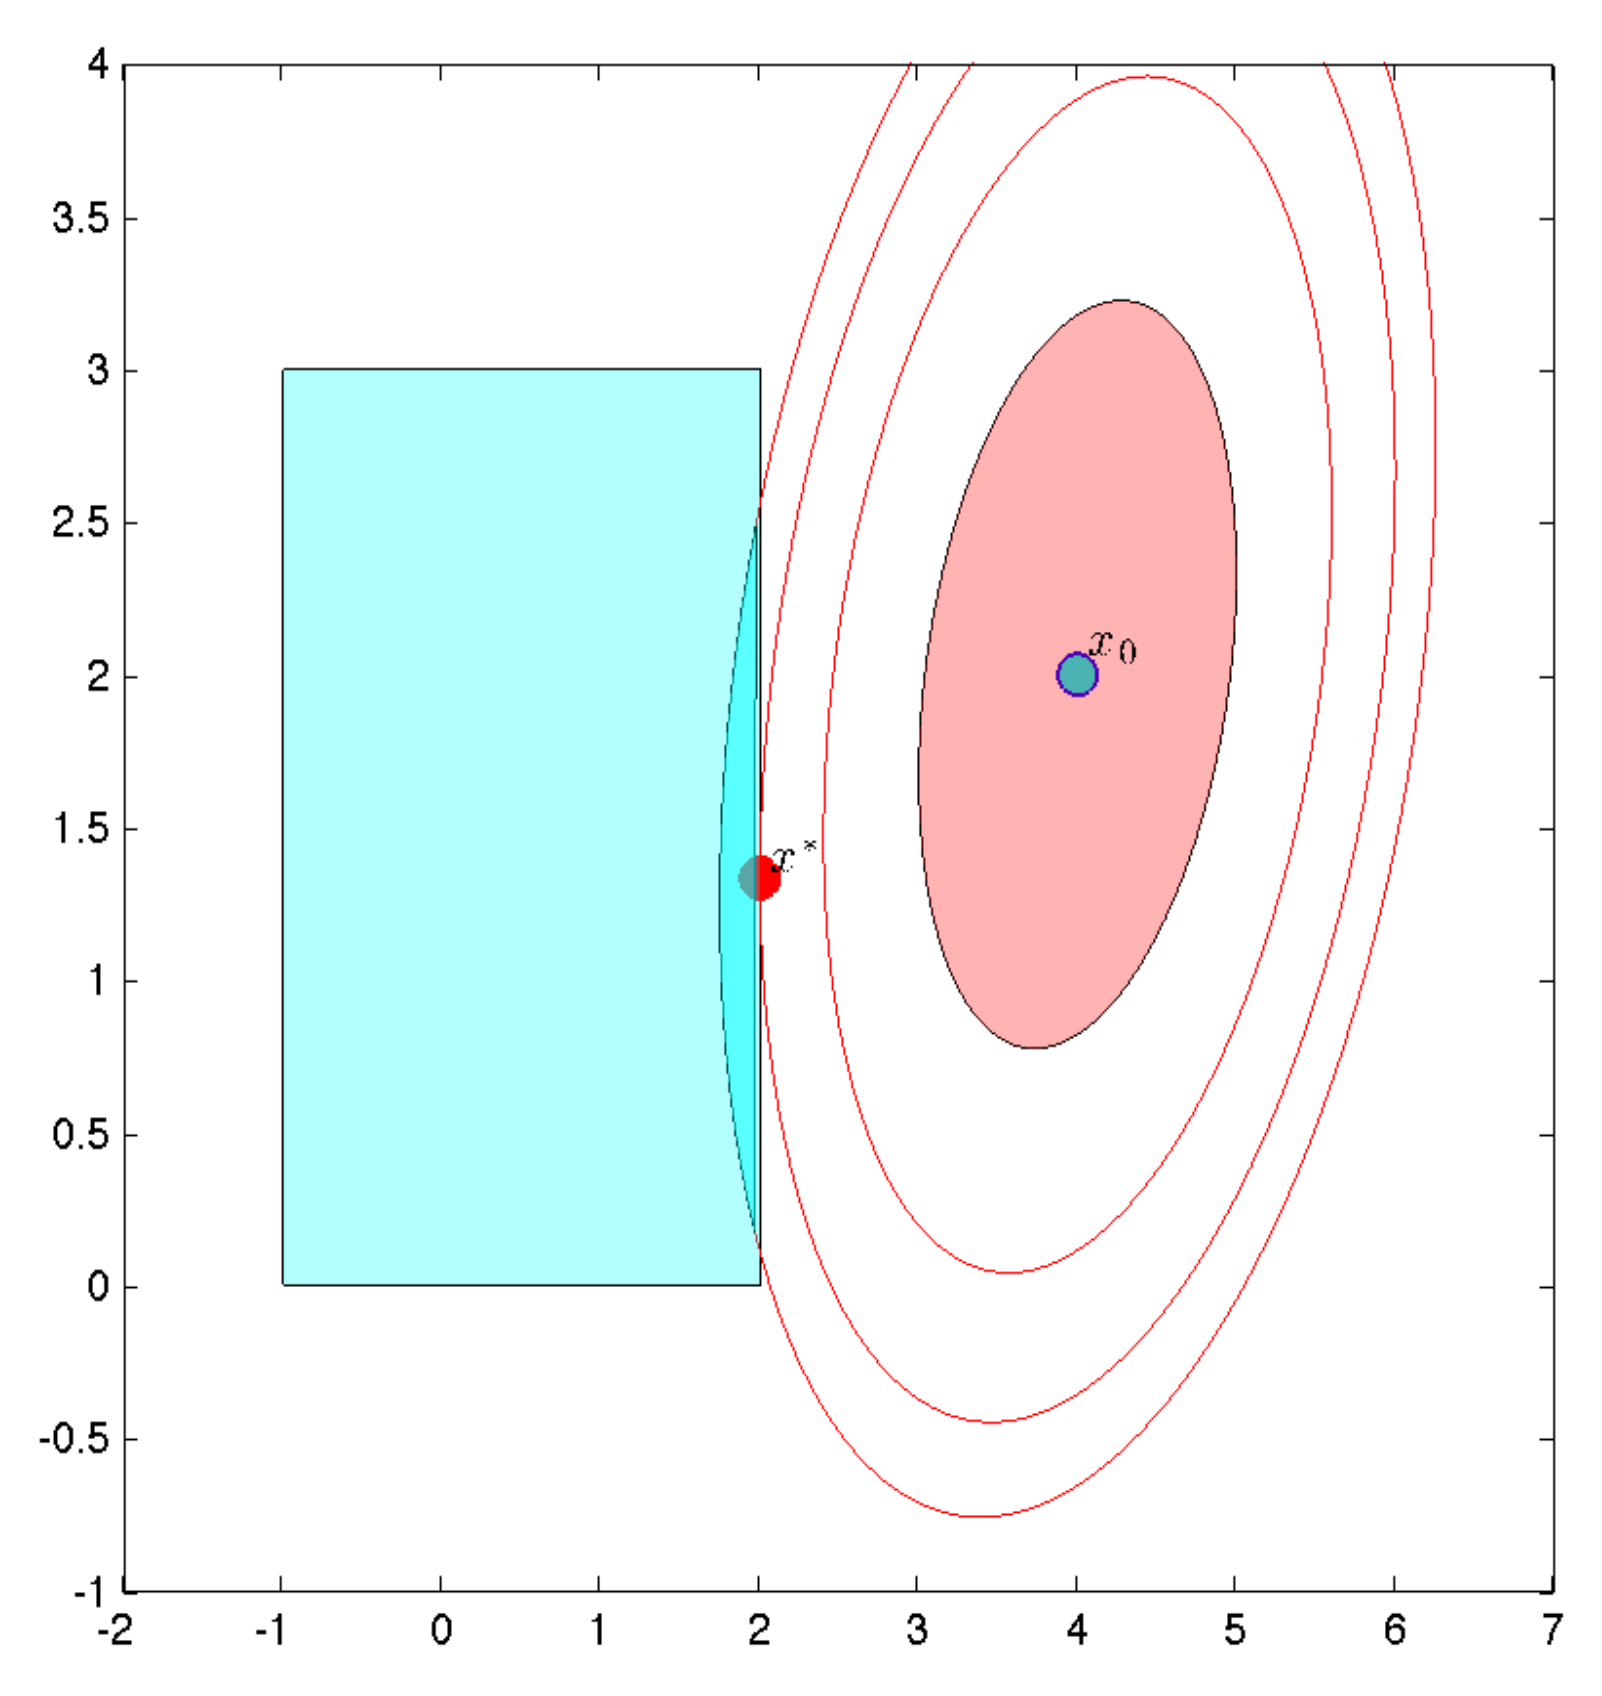
\includegraphics[scale=0.3]{figures/optexamplebasic}\caption{Optimization Problem Definitions Example}\end{center}\end{figure}
\end{example}
\begin{itemize}
\item The feasible set is in light blue.
\item The $0.1$-suboptimal set is in darker blue.
\item The unconstrained minimizer is $x_0$. This is the solution to the optimization problem without any constraints applied.
\item The optimal point is $x^*$.
\item The level sets of the objective function are the red lines.
\item The sub-level set is the filled in red ellipse.
\item The optimal value $p^*=-10.2667$ is attained by the optimal solution $x_1^*=2, x_2^*=1.3333$.
\end{itemize}
\subsection{Convex Problems}
Recall the graph in Figure 4 where we had multiple local minima. As we saw, this is a hard case to deal with. However, there is a class of optimization problems that don't face this issue of multiple local minima. This class contains optimization problems where the objective function and constraints involve convex functions. 
\subsubsection{What does it mean to be convex?}
Roughly speaking, a convex function has \textit{bowl-shaped} graph:
\begin{figure}[h!]\begin{center}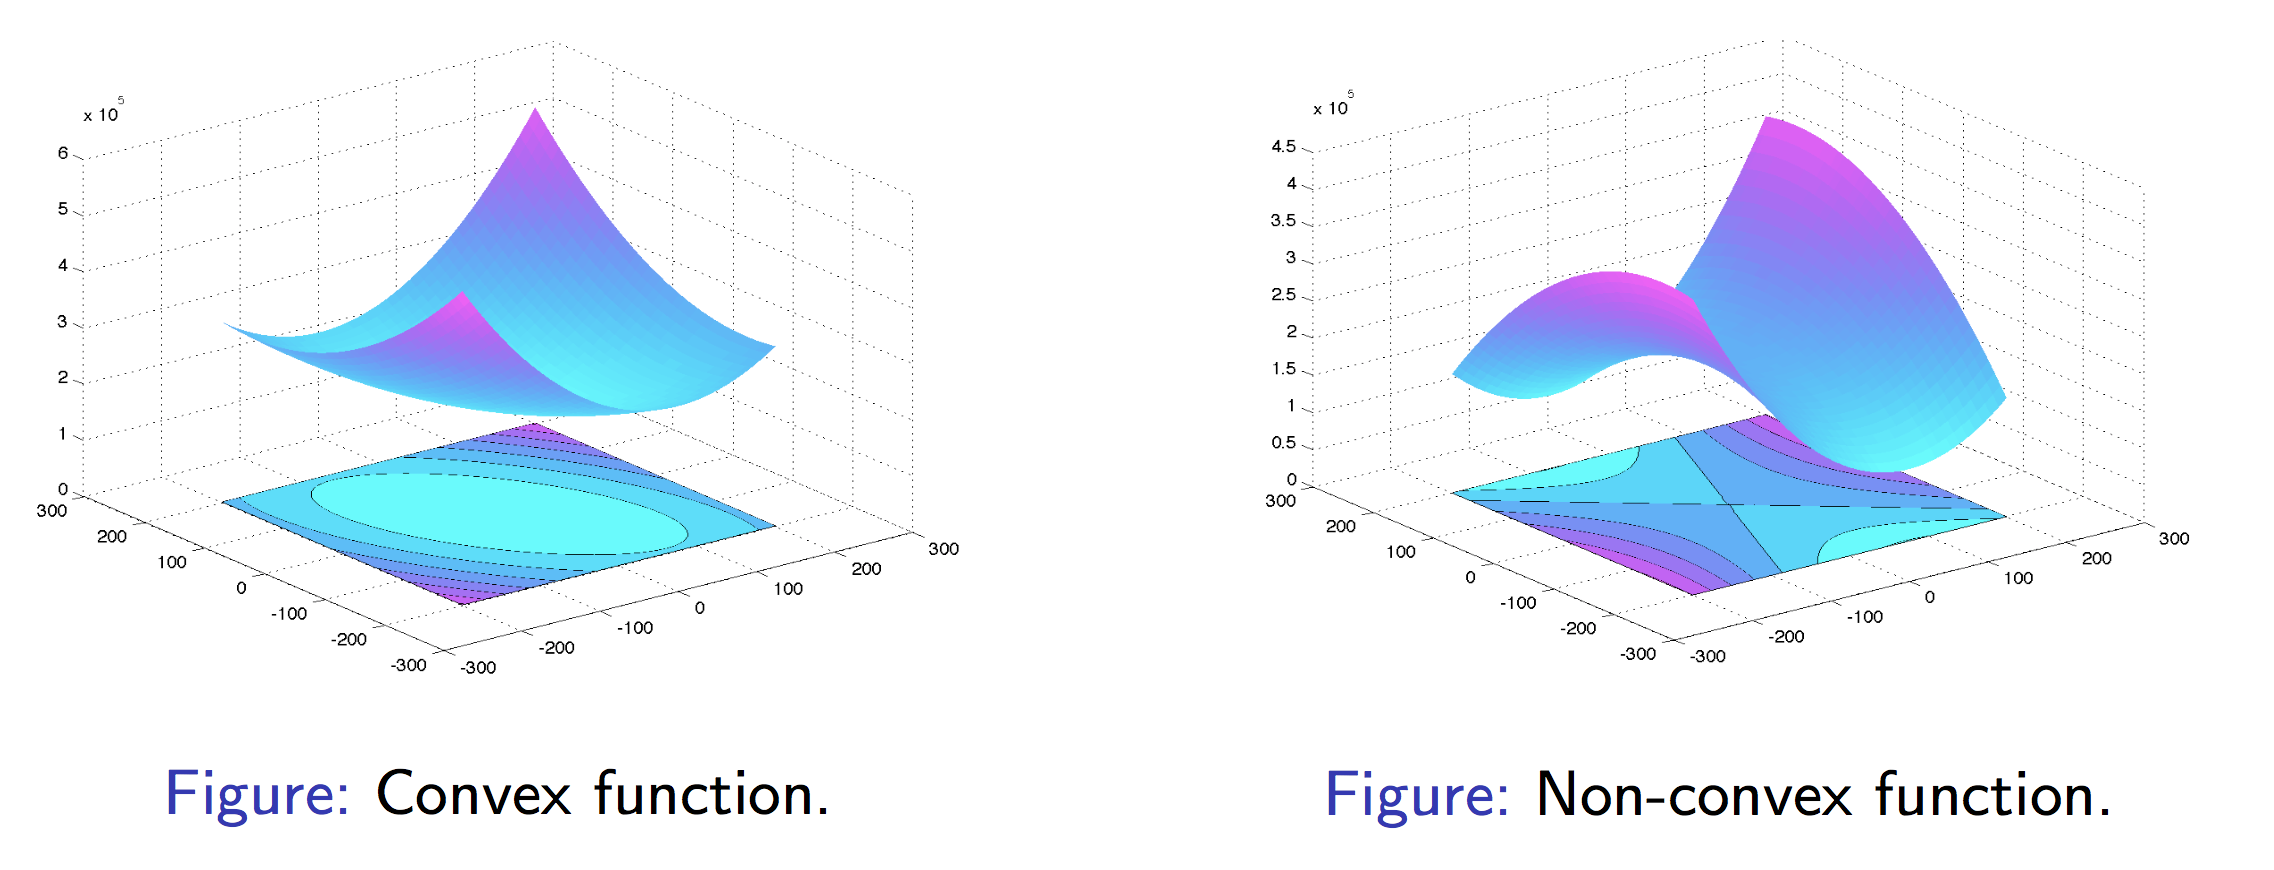
\includegraphics[scale=0.35]{figures/convex}\caption{An Example of a Convex and Non-convex Function}\end{center}\end{figure}
\begin{definition}
A set $E\subset \mathbb{R}^n$ is convex if $$\lambda\mathbf{x} +(1-\lambda)\mathbf{y}\in E$$ whenever $\mathbf{x},\mathbf{y}\in E$ and $0<\lambda<1$.
\end{definition}
\noindent Loosely, this definition is saying that if a function is convex and I draw a line from one point to another point on that function, the line will always lie inside the function. 
\begin{figure}[h!]\begin{center}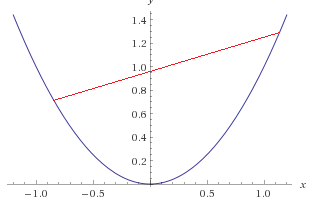
\includegraphics[scale=0.45]{figures/convfunc}\caption{A Convex Function}\end{center}\end{figure}

\noindent Notice, in Figure 7, how the red line lies inside the parabola. If this is true for any two points on the function, the function is said to be convex. One of the key features of convex functions is that all local minima are global minima. Recall the function in Figure 3. This function was also convex, with multiple global minima.

\noindent When dealing with a convex optimization problem, optimization becomes very reliable. In the past 50 years, many people have been working on solving linear equations at scale. Now, modules and functions in Python and Matlab can reliably solve linear equations. Instead of worrying about whether or not an algorithm in Python found the solution, we have reached the point where we can consider it a reliable black box. 

\noindent Convex optimization is similar. It is very reliable to solve an optimization problem where we know the objective function and it's constraints to involve convex functions. However, not all convex problems are easy to solve. In this course, we will mostly deal with convex optimization.

\subsubsection{Special Convex Models}
In this course, we will deal specifically with convex optimization problems with special structure, such as:
\begin{itemize}
\item Least-Squares (LS)
\item Linear Programs (LP)
\item Convex Quadratic Programs (QP)
\item Second-order Cone Programs (SOCP)
\end{itemize}
We will utilize certain software (such as CVX, Yalmip, Mosek, etc.) which contain efficient algorithms, to solve such optimization problems.
\subsection{Non-convex Problems}
There are three main types on Non-convex optimization problems:
\subsubsection{Boolean/Integer Optimization}
Suppose that we are an airline company that is trying to allocate resources: pilots, flight attendants, etc.. Now, suppose that we want to send some pilots and flight attends to airplanes based on demand, traffic, etc. However, notice that there is another layer of complexity in this problem: we cannot send half a pilot to an airplane. Here, we are facing a boolean optimization problem. Solving such problems is hard. 
\subsubsection{Cardinality-Constrained Problem}
Here we seek to bound the number of non-zero elements in a vector variable.
\subsubsection{Non-linear Programming}
These consist of non-convex problems with differentiable objective function. 

\nocite{*}
\bibliographystyle{alpha}
\bibliography{refs}

\end{document}
